\section{Exercício 1}

Considere o experimento computacional denominado “Polynomial Curve Fitting”, usado
diversas vezes no livro texto (veja páginas 4 e 5 do livro, bem como Apêndice A), considerando a
ordem do modelo sendo M = 9 e o tamanho da amostra sendo N = 10.
Faça:

\begin{enumerate}[label=(\alph*)]
    \item Calcule a solução de mínimos quadrados (LS) \( \mathbf{w_{LS}} \);
    \item Calcule a solução via regressão ridge (escolha um fator de regularização razoável) \( \mathbf{w_{ridge}} \);
    \item Calcule a solução via regressão lasso (escolha um fator de regularização razoável) \( \mathbf{w_{lasso}} \);
    \item Monte uma tabela exibindo os 10 coeficientes \( \mathbf{w} \) para as 3 soluções obtidas nos itens acima e comente/compare os resultados;
    \item Plote uma figura contendo o processo gerador em verde (a senoide), e suas estimativas \( y_{LS} \), \( y_{ridge} \), e \( y_{lasso} \) em preto, azul e vermelho, respectivamente;
    \item Repita todos os itens anteriores para \( N=20 \) e \( N=50 \).
\end{enumerate}

\subsection{Resposta do item (a)}
Para responder esse item foi utilizada a classe $LinearRegression()$ da biblioteca \textit{sklearn} para linguagem \textit{Python}, que realiza uma regressão linear utilizando mínimos quadrados. Foi escolhido um polinômio de ordem 9 como modelo.
\begin{figure}[H]
    \centering
    \caption{Solução para mínimos quadrados (LS)}
    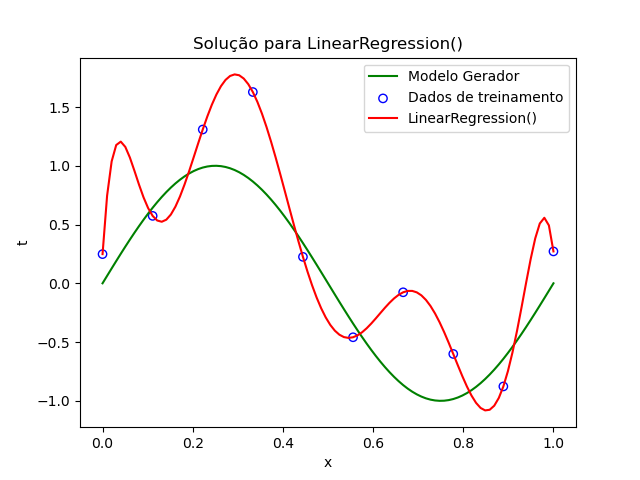
\includegraphics[width=12cm]{E1_a.png}
\end{figure}
A regressão linear por mínimos quadrados não introduz nenhuma regularização e por isso a curva vermelha passa exatamente pelos dados de treinamento, mostrando que eles foram decorados overfitting.


\subsection{Resposta do item (b)}
Para responder esse item foi utilizada a classe $Ridge()$ da biblioteca \textit{sklearn} para linguagem \textit{Python}, que realiza uma regressão linear utilizando mínimos quadrados e regularização de norma $L_2$ (Ridge). Foi escolhido um polinômio de ordem 9 como modelo e o fator de regularização $\lambda$, que na classe $Ridge()$ é chamado de \textit{alpha}, que melhor adaptou a curva ao modelo gerador foi $1^{-0.5}$.
\begin{figure}[H]
    \centering
    \caption{Solução para Ridge com $\lambda = 1^{-0.5}$}
    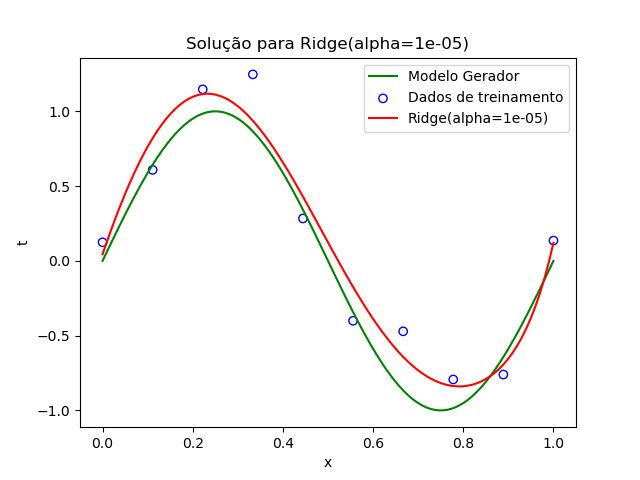
\includegraphics[width=12cm]{E1_b.png}
\end{figure}
A regressão Ridge introduz uma penalização nos coeficientes através do fator de regularização, ajudando a evitar overfitting.

\subsection{Resposta do item (c)}
Para responder esse item foi utilizada a classe $Lasso()$ da biblioteca \textit{sklearn} para linguagem \textit{Python}, que realiza uma regressão linear utilizando mínimos quadrados e regularização de norma $L_1$ (Lasso). Foi escolhido um polinômio de ordem 9 como modelo e o fator de regularização $\lambda$, que na classe $Lasso()$ é chamado de \textit{alpha}, que melhor adaptou a curva ao modelo gerador foi $1^{-0.5}$.
\begin{figure}[H]
    \centering
    \caption{Solução para Lasso com $\lambda = 10^{-0.6}$}
    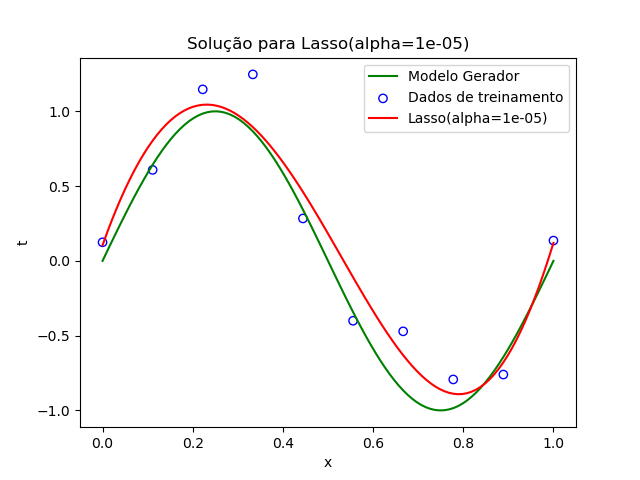
\includegraphics[width=12cm]{E1_c.png}
\end{figure}
A regressão Lasso, assim como a Ridge, introduz uma penalização nos coeficientes através do fator de regularização, ajudando a evitar overfitting.

\subsection{Resposta do item (d)}

A tabela abaixo exibindo os coeficientes para as três soluções permite comparar diretamente o impacto da regularização nos coeficientes.

\begin{table}[H]
    \caption{Coeficientes para $N=10$}
    \centering
    \begin{tabular}{|l|lll|}
        \toprule
        Modelo & LS & Ridge & Lasso \\
        \midrule
        $w_0$ & 0.00000 & 0.00000 & 0.00000 \\
        $w_1$ & 61.35162 & 5.57635 & 7.87333 \\
        $w_2$ & -1305.39950 & -10.39014 & -18.23029 \\
        $w_3$ & 10864.20021 & -3.32097 & 2.98646 \\
        $w_4$ & -43958.48661 & 2.24588 & 5.01574 \\
        $w_5$ & 96013.72998 & 3.46376 & 2.15551 \\
        $w_6$ & -116795.01934 & 2.37258 & 0.11133 \\
        $w_7$ & 75859.90079 & 0.81213 & 0.00000 \\
        $w_8$ & -22103.99856 & -0.27544 & -0.00000 \\
        $w_9$ & 1363.74433 & -0.58096 & 0.08759 \\
        \bottomrule
    \end{tabular}
\end{table}

A regressão por mínimos quadrados sem regularização tende a produzir coeficientes maiores, um dos sinais que indicam overfitting ou pelo menos uma alta sensibilidade aos dados de treinamento. Enquanto que os coeficientes produzidos pela Ridge e pela Lasso são menores.

Além disso, é possível observar a presença de alguns coeficientes praticamente nulos para a Lasso. Esse resultado era esperado, uma vez que a Lasso, por utilizar a norma $L_1$, tende a produzir uma solução mais esparsa, selecionando atributos mais importantes.

Enquanto isso, a regressão Ridge, apesar de não selecionar atributos como a Lasso, tende a penalizar ainda mais os coeficientes grandes, consequentemente fazendo com que os maiores coeficientes fiquem menores que os produzidos pela Lasso.



\subsection{Resposta do item (e)}
\begin{figure}[H]
    \centering
    \caption{Comparação entre as soluções para $N=10$}
    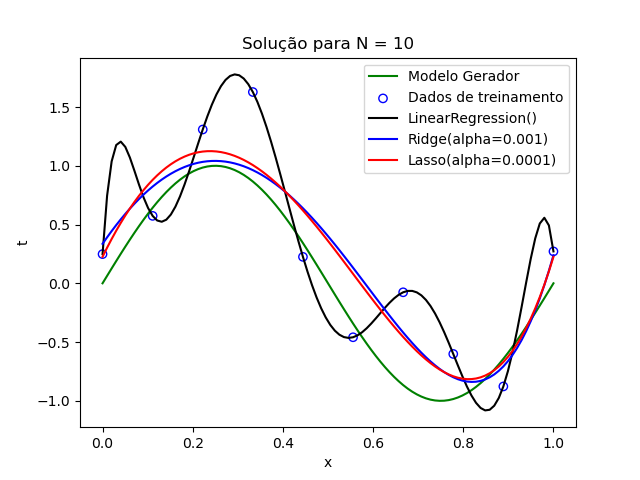
\includegraphics[width=12cm]{E1_e.png}
\end{figure}

\subsection{Resposta do item (f)}

\begin{figure}[H]
    \centering
    \caption{Comparação entre as soluções para $N=20$}
    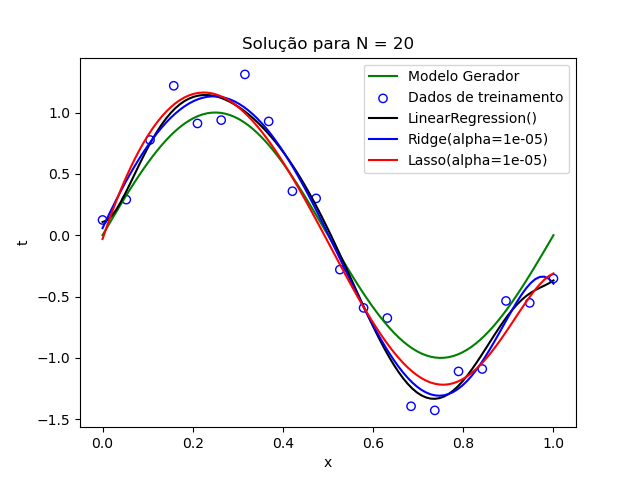
\includegraphics[width=12cm]{E1_f20.png}
\end{figure}
\begin{table}[H]
    \caption{Coeficientes para $N=20$}
    \centering
        \begin{tabular}{|l|lll|}
            \toprule
            Modelo & LS & Ridge & Lasso \\
            \midrule
            $w_0$ & 0.00000 & 0.00000 & 0.00000 \\      
            $w_1$ & -6.01368 & 8.39435 & 12.41611 \\    
            $w_2$ & 266.50406 & -16.21245 & -29.59271 \\
            $w_3$ & -2042.90037 & -8.39927 & 0.72172 \\ 
            $w_4$ & 7178.62334 & 2.98152 & 10.38544 \\  
            $w_5$ & -13245.77187 & 9.30126 & 8.97546 \\ 
            $w_6$ & 11993.83639 & 9.76174 & 4.54743 \\
            $w_7$ & -3017.56404 & 5.62434 & 0.00000 \\
            $w_8$ & -2424.08815 & -1.60172 & -1.35976 \\
            $w_9$ & 1296.42241 & -10.65716 & -6.72254 \\
            \bottomrule
        \end{tabular}
\end{table}


\begin{figure}[H]
    \centering
    \caption{Comparação entre as soluções para $N=50$}
    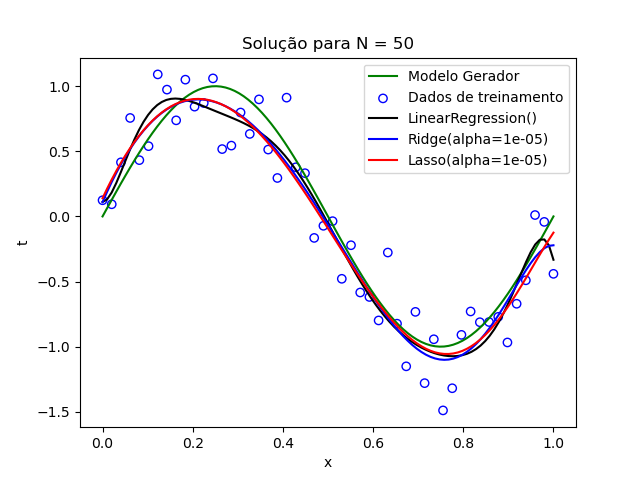
\includegraphics[width=12cm]{E1_f50.png}
\end{figure}

\begin{table}[H]
    \caption{Coeficientes para $N=50$}
    \centering
        \begin{tabular}{|l|lll|}
            \toprule
            Modelo & LS & Ridge & Lasso \\
            \midrule
            $w_0$ & 0.00000 & 0.00000 & 0.00000 \\
            $w_1$ & -6.39374 & 4.21035 & 5.11672 \\
            $w_2$ & 455.99223 & -10.53780 & -14.48266 \\
            $w_3$ & -5270.52166 & -3.22874 & 0.35582 \\
            $w_4$ & 27669.16750 & 1.83804 & 4.73458 \\
            $w_5$ & -80097.04531 & 4.61815 & 4.18727 \\
            $w_6$ & 135776.45582 & 5.20904 & 2.22228 \\
            $w_7$ & -134351.92251 & 3.52870 & 0.00000 \\
            $w_8$ & 71926.93850 & -0.30771 & -0.00000 \\
            $w_9$ & -16103.55817 & -6.01761 & -2.73785 \\
            \bottomrule
        \end{tabular}
\end{table}


Pelas figuras, podemos observar que a solução para mínimos quadrados começa a sofrer menos com o overfitting à medida que o tamanho da amostra aumenta. Isso se deve ao fato de que o ruído nos dados de treinamento possui uma distribuição gaussiana com média zero. Pela lei dos grandes números, quanto maior a quantidade de dados de treinamento, mais a média da amostra se aproxima da média da distribuição original, que é zero, reduzindo assim o efeito do ruído.

Consequentemente, com mais dados, a solução de mínimos quadrados consegue capturar melhor o padrão subjacente dos dados, e o impacto do ruído diminui. Esse comportamento explica por que a solução de mínimos quadrados apresenta um ajuste mais estável e menos propenso ao overfitting quando o tamanho da amostra aumenta.

No entanto, é importante notar que, mesmo com um aumento no tamanho da amostra, métodos de regularização como a regressão ridge e lasso continuam a fornecer soluções mais robustas e generalizáveis, especialmente em situações onde o ruído pode não ser perfeitamente gaussiano ou quando a complexidade do modelo ainda é alta em relação ao tamanho da amostra.






